\documentclass[12pt]{article}
\pagestyle{empty}
\setlength{\parskip}{0in}
\setlength{\textwidth}{6.8in}
\setlength{\topmargin}{-.5in}
\setlength{\textheight}{9.3in}
\setlength{\parindent}{0in}
\setlength{\oddsidemargin}{-.7cm}
\setlength{\evensidemargin}{-.7cm}

\usepackage{amsmath}
\usepackage{amsthm}
\usepackage{amstext}

\usepackage{graphicx}

\begin{document}

\emph{As you work on this practice exam, keep a running ``don't forget'' list of any information you need to look up or ask about.}
\bigskip

\subsection*{Practice exam 1 -- IN-CLASS VERSION}
\bigskip

Relax.  You have done problems like these before.  Even if these problems look a bit different, just do what you can.  If you're not sure of something, please ask! You may use your calculator.  Please show all of your work and write down as many steps as you can.  Don't spend too much time on any one problem.  Do well.  And remember, ask me if you're not sure about something.
 
 \begin{center}

\begin{tabular}
{|l|c|c|c|c|c|c|c|c|c|c|c|c||c|c} \hline

 Problems & \hspace{5 pt} 1 \hspace{5 pt}  & \hspace{5 pt} 2 \hspace{5 pt} & \hspace{5 pt} 3 \hspace{5 pt} & \hspace{5 pt} 4 \hspace{5 pt}  & \hspace{5 pt} Subtotal  \hspace{5 pt} & +DQ& Total &\hspace{5 pt} Grade \hspace{5 pt}  \\ \hline
&&&&&&&&\\  
Points &&&&&&&   \hspace{.8in}\% &  \\ 
&&&&&&&& \\  \hline
Out of & 30 & 35 & 15 & 20  &100 & (max 5)& & \\ \hline
\end {tabular}

\end{center}

\vfill

\newpage  %% EXAM STARTS HERE

\begin{enumerate}
%\item Dakota got a parking ticket.  It's only \$20 but they add an extra \$5 per week if he pays late.
%\begin{enumerate}
%\item Name the variables, including units and dependence. 
%\item If Dakota pays the ticket two weeks late, what will he owe?
%\item Dakota totally forgot about the ticket.  But then he received a summons from the county clerk's office:  either pay the ticket (now \$100) or go to court.  How many weeks late is it?
%\item Make a table of the values you found so far.
%\item Draw a graph showing how Dakota's parking ticket increases over time.
%\end{enumerate}
 
 \item Arva and Ellie began hiking at an elevation of \text{1,500} feet and climbed at the steady rate of 600 vertical feet per hour. % was Benji
\begin{enumerate}
\item Make a table showing their elevation after 1 hour, 2 hours, and 5 hours. \vfill \vfill
\item Name the variables, including units. \vfill \vfill
\item Explain the dependence using a sentence of the form ``\underline{~\quad} is a function of \underline{~\quad}.'' \vfill
\item Is the function increasing or decreasing? \vfill
\item How long does it take them to reach \text{5,300} feet up?  Try to figure out the answer in hours and minutes (H:MM format). \vfill \vfill \vfill
\end{enumerate}


\newpage

\item The table shows Henry's weight as a baby.
\begin{center}
\begin{tabular} {|l||c|c|c|} \hline
Age (weeks) & 0 & 12 & 15 \\ \hline
Weight (pounds) & 8 & 14 & 16 \\ \hline
\end{tabular}
\end{center}
\begin{enumerate}
\item How much weight did Henry gain, on average, each week during his first 12 weeks? \vfill
\item During which time interval was Henry gaining weight faster?  \emph{Explain.} \vfill
 \item Identify the variables, including units and dependence. \vfill
 \item Draw a graph illustrating the dependence.  Choose a scale that shows up to 20 weeks and 20 pounds. \bigskip
\begin{center}
\scalebox {.8} {
\includegraphics [width = 6in] {GraphPaper.jpg}}
\end{center}

\bigskip
\item What might you guess for Henry's weight at 20 weeks?   \vfill
\end{enumerate} 

\newpage

%\item (1.4) August 2012.  London.  The United States Olympic team set a new record in the women's 4$\times$100 relay with a time of 40.82 seconds.
%\hfill \begin{footnotesize} Source:  Wikipedia (4$\times$100 metres relay) \end{footnotesize}
%\begin{enumerate}
%\item The race totals 400 meters.  How fast did the women run, as measured in meters/sec?  
%\item Convert their speed to mph.   Use that $1 \text{ mile} \approx {1,609} \text{ meters}$.
%\end{enumerate}

\item Pramesh's new car used 20.5 gallons of gas for a 715 mile trip. 
\begin{enumerate}
\item How many miles per gallon (mpg) does his car get? \vfill
\item At that rate, how many gallons of gas would Pramesh use on his 3,200 mile cross-country trip?  \vfill
\item If gas costs \$3.799/gallon, how much will gas for that trip cost?  \vfill
%\item Make a table of values showing the cost for gas for Pramesh's trip if gas costs \$3.599/gal, \$3.599/gal, \$3.799/gal, or \$3.899/gal. 
%\item Identify the variables and constants (if any) suggested by the previous question.  As always, include the units, realistic domain, and dependence. 
\end{enumerate}

\newpage

\item Ndwiga is reading an article in the paper about atoms.  From his physics textbook he discovered that the size of an atom is .142 nanometers.  (That's 0.142 nanometers.)
\begin{enumerate}
\item Write the size of an atom in meters.  Use $1 \text{ meter} = \text{1,000,000,000 nanometers}$.   Write your answer in usual decimal notation and in scientific notation. \vfill \vfill
\item Ndwiga would like to know how many atoms across this sheet of paper which is 8.5 inches wide. Use that $1 \text{ inch} \approx 2.54 \text{ cm}$ and $1 \text{ meter} = 100 \text{ cm}$.  Express your final answer in billions of atoms. \vfill \vfill \vfill
\end{enumerate}

%%%% END

\end{enumerate}

\newpage %% OTHER VERSION GOES HERE!

\emph{Try taking this take-home version of the practice exam under testing conditions:  no book, no notes, no classmate's help, no electronics (computer, cell phone, television). Give yourself one hour to work and wait until you have tried your best on all of the problems before checking any answers.}
\bigskip  %UNDO

\subsection*{Practice exam 1 -- TAKE HOME VERSION}
\bigskip

Relax.  You have done problems like these before.  Even if these problems look a bit different, just do what you can.  If you're not sure of something, please ask! You may use your calculator.  Please show all of your work and write down as many steps as you can.  Don't spend too much time on any one problem.  Do well.  And remember, ask me if you're not sure about something.
 
 \begin{center}

\begin{tabular}
{|l|c|c|c|c|c|c|c|c|c|c|c|c||c|c} \hline

 Problems & \hspace{5 pt} 1 \hspace{5 pt}  & \hspace{5 pt} 2 \hspace{5 pt} & \hspace{5 pt} 3 \hspace{5 pt} & \hspace{5 pt} 4 \hspace{5 pt} &  \hspace{5 pt} Subtotal  \hspace{5 pt} & +DQ& Total &\hspace{5 pt} Grade \hspace{5 pt}  \\ \hline
&&&&&&&&\\  
Points &&&&&&&   \hspace{.8in}\% &  \\ 
&&&&&&&& \\  \hline
Out of & 18 & 32 & 28 & 22 &100 & (max 5)& & \\ \hline
\end {tabular}

\end{center}

\vfill

\newpage %UNDO  
 %% EXAM STARTS HERE

\begin{enumerate}

\item The amount of money spent on nursing home care for seniors has continued to rise.  The table shows the values for select years.  Here $S$ is the spending, measured in billions of dollars and $Y$ is the year, measured in years since 1960.
%The amount of money in nursing home care $C$, in billions of dollars since 1960 is approximated by the equation $$C = 0.07214Y^2-0.4957Y+1.029$$
%where $Y$ is the year since 1960, and $C$ is the money spent on care in biollions of dollars.

\begin{center}
\begin{tabular} {|c ||c |c |c |c |c |c |c |} \hline
%year & 1960 & 1970 & 1985 & 2000 & 2012 \\ \hline
$Y$ & 0 & 10 & 25 & 40 & 52 \\ \hline
$S$ & 1.0 & 3.3 & 33.7 & 96.6 & 170.3 \\ \hline
\end{tabular}
\end{center}

\begin{enumerate}
\item According to the table, what was the spending in 1970?  \vfill
\item According to the table, what was the spending in 1985?  \vfill
\item Calculate the rate of change of spending over the period 1970 to 1985.  Don't forget to state the units. \vfill \vfill
\item In approximately what year did spending first pass \$50 billion? \vfill
\end{enumerate}

\newpage

\item Trish is filling a swimming pool with water.  The graph below shows how many gallons of water ($G$) are in the pool after $H$ hours.  Use the graph to answer the following questions.
\begin{center}
\scalebox {.9} {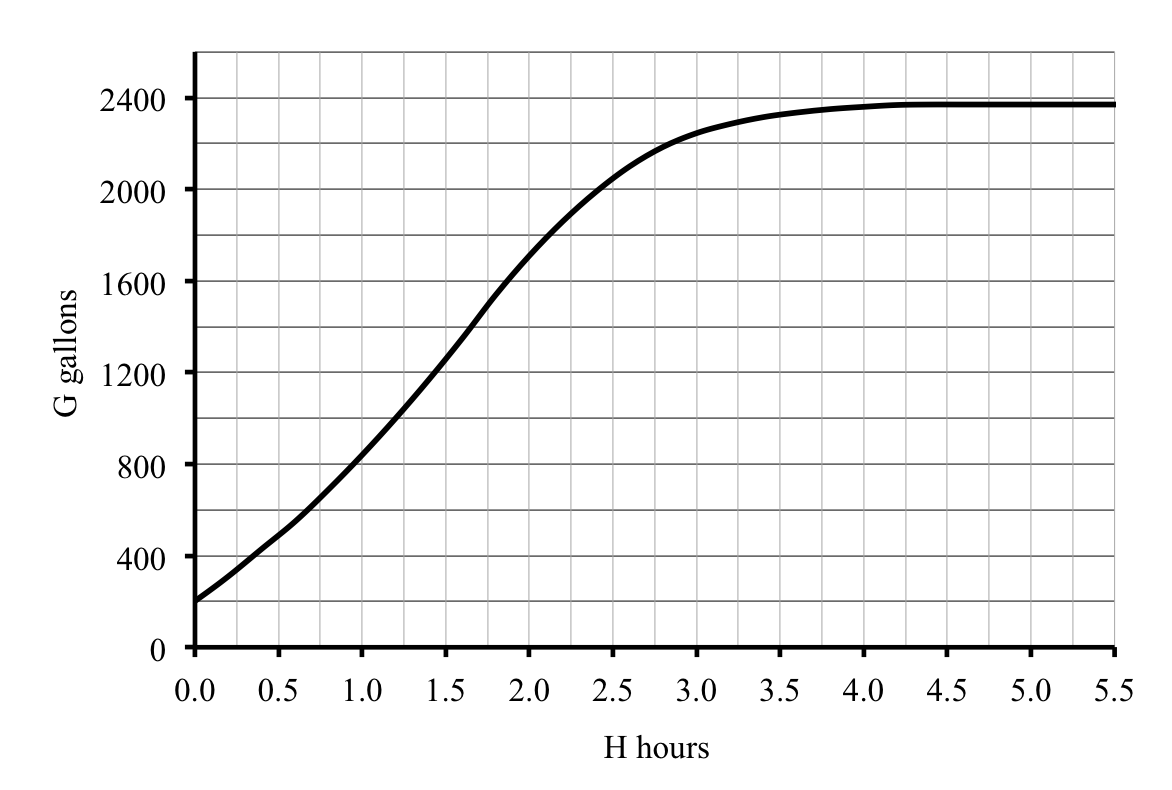
\includegraphics [width = 6in] {fillingtankNEW}}
\end{center} 
\begin{enumerate}
\item How much water was in the swimming pool already when Trish began? \vfill
\item How much water was in the swimming pool after 3 hours? \vfill
\item After how many hours were there \text{1,000} gallons of water in the swimming pool? \vfill
\item Was Trish filling the pool faster at 2 hours or at 2.5 hours?  Explain how you see that on the graph. \vfill
\item After (about) how many hours did Trish stop filling the swimming pool?  Explain how you see that on the graph. \vfill
\end{enumerate}

\newpage

\item In 1990 the Lef\`evre's property tax was \$450 but it doubled every year thereafter.  
 \begin{enumerate}
 \item Name the variables, including units. \vfill \vfill
 \item Which is the independent variable and which is the dependent variable? \vfill
\item Make a table showing the property tax each year from 1990 to 1994. \vfill \vfill
\item Draw a graph illustrating the dependence.
\bigskip
\begin{center}
\scalebox {.8} {
\includegraphics [width = 6in] {GraphPaper.jpg}}
\end{center}
\bigskip
%\item Looking at your graph, do you think property taxes increased at this rate through 2000?  (In fact, the city provided rebates to property owners with fast-rising taxes starting in 1994.)
 \end{enumerate} 
 
\newpage

\item The distance from the Earth to the Moon is approximately \text{384,000,000} meters. 
%\hfill \begin{footnotesize} Source:  Wikipedia (Lunar distance)\end{footnotesize}
\begin{enumerate}
\item Express this distance in scientific notation. \vfill
\item Express this distance in kilometers (km), using $1 \text{ km} = \text{1,000 meters}$. \vfill
\item Express this distance in miles, using the conversion $1 \text{ mile} \approx 1.609 \text{ km}$. \vfill
\item If you could drive to the moon at 55 mph, how long would it take to get there? Express your answer in terms of months, using $1 \text{ month} \approx 30 \text{ days}$. \vfill
\end{enumerate}


%%%% END

\end{enumerate}


\end{document}

